\documentclass[pdflatex,compress]{beamer}

%\usetheme[dark,framenumber,totalframenumber]{ElektroITK}
\usetheme[darktitle,framenumber,totalframenumber]{ElektroITK}
\usepackage[utf8]{inputenc}
\usepackage[T1]{fontenc}
\usepackage{lmodern}
%\usepackage[bahasai]{babel}
\usepackage{amsmath}
\usepackage{amsfonts}
\usepackage{amssymb}
\usepackage{graphicx}
\usepackage{multicol}
\usepackage{lipsum}
\usefonttheme[onlymath]{serif}

\newcommand*{\Scale}[2][4]{\scalebox{#1}{$#2$}}%

\setbeamertemplate{caption}[numbered]

\AtBeginSection[]{
	\begin{frame}
		\vfill
		\centering
		\usebeamerfont{title}\insertsectionhead\par%
		\vfill
	\end{frame}
}

\title{Electronic Circuit II}
\subtitle{Differential Amplifier}
\author{Mifta Nur Farid}
\date{16 March 2023}

\begin{document}

\maketitle

\begin{frame}
	\frametitle{Differential Amplifier}
	\begin{center}
		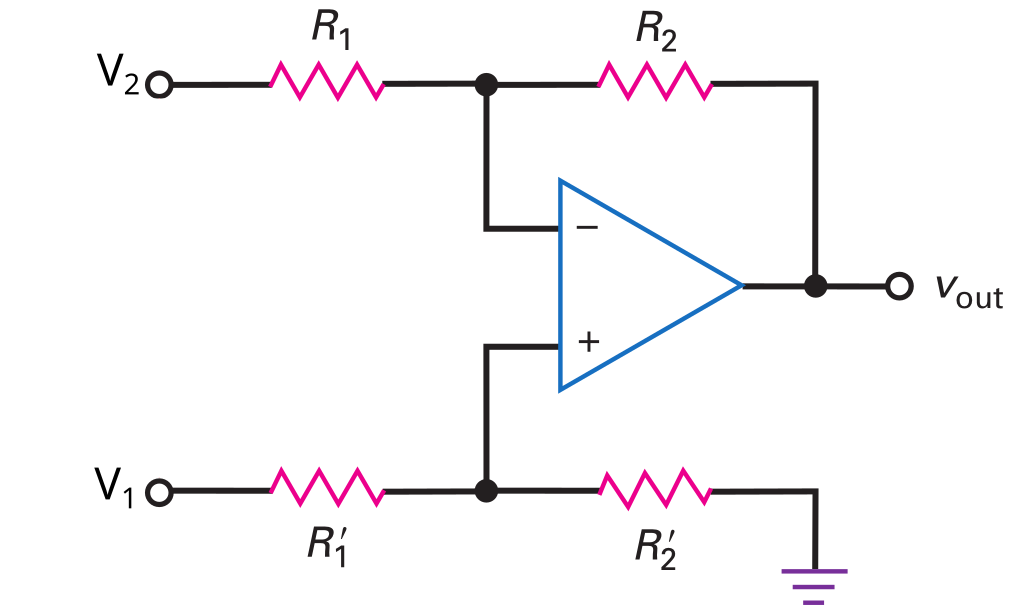
\includegraphics[width=0.8\linewidth]{img/Figure-18-14a}
	\end{center}
\end{frame}

\begin{frame}{Differential Amplifier}

\end{frame}

\end{document}
